\documentclass[journal,letterpaper]{IEEEtran}
\usepackage[letterpaper, left=0.65in, right=0.65in, bottom=0.7in, top=0.7in]{geometry}
\usepackage{stix}
\usepackage{siunitx}
\usepackage[version=4]{mhchem}
\usepackage{booktabs}
\usepackage{makecell}
\usepackage{multirow}
\usepackage{amsmath}
\usepackage{bm}
\usepackage{graphicx}
\usepackage{tikz}
\usepackage{pgfplots}
\usepackage{float}
\usepackage{fancyhdr}
\usepackage[none]{hyphenat}
\usepackage[hidelinks]{hyperref}
\usepackage{import}
\usepackage{transparent}
\usepackage{microtype}

\graphicspath{ {./figures/} }

\pgfplotsset{compat=1.18}

\setlength{\columnsep}{0.2in}
\setlength{\columnwidth}{3.5in}

\newlength\fheight
\newlength\fwidth
\setlength\fwidth{3.25in}
\setlength\fheight{0.8\fwidth}

\newcommand{\incfig}[1]{%
    \centering
    \def\svgwidth{3.5in}
    \import{./figures/}{#1.pdf_tex}
}

\sisetup{per-mode = symbol, inter-unit-product = \ensuremath{ { } \cdot { } }, number-unit-product = \text{ }}

\pagestyle{fancy}
\fancyhf{}
\renewcommand{\headrulewidth}{0pt}
\rhead{\thepage}
\lhead{Section 11832 Lab 1}

\begin{document}
\title{Determining a Wind Tunnel Calibration Coefficient to Predict the Fluid Velocity and Velocity Profile}

\author{\IEEEauthorblockN{\huge{Borg, Auston J. \\ Lam, Brandon H. \\ Latzko, Alexander J. \\}}
\IEEEauthorblockA{
Section 11832 \quad September 19, 2023}
}

\maketitle
\thispagestyle{empty}

\begin{abstract}
This study presents a method of determining airspeed or dynamic pressure when unfavorable Pitot-static probe conditions are present in addition to characterizing the velocity profile of a given wind tunnel.
A pressure transducer is first calibrated using a water manometer to properly measure gauge pressures.
The calibrated pressure transducer and Pitot-static probe are used to measure the dynamic and change in static pressure at differing fan speeds in the empty test section.
It can be shown from the first law of thermodynamics that the dynamic pressure and the change in static pressure should be proportional.
After the experimental data was analyzed, a tunnel calibration constant of $\bm{K = -0.600 \pm 0.002}$ was derived.
The Pitot-static probe was then used to measure the dynamic pressure at varying heights in the test section to define the velocity profile.
It was found that the velocity profile exhibited signs of uniform flow with sharp decreases in velocity at the walls.
This velocity profile pattern was common for the entrance and exit of the test section.
\end{abstract}

\begin{IEEEkeywords}
calibration, flow velocity, viscous loss, wind tunnel
\end{IEEEkeywords}


\section{Introduction}


\IEEEPARstart{W}{ind} tunnels have proven to be a valuable tool for predicting the aerodynamic capabilities of objects for over a century~\cite{lecture}.
Air is moved through the tunnel and the interactions between the airflow and a scale model can be used to simulate the actual characteristics of the object in flight.
As the velocity of the flowing air can be a major influence on the aerodynamics of the object in the wind tunnel, it is vital to have an accurate understanding of the velocity of the airflow.
This can be complicated by the presence of viscous losses and the use of flow conditioning screens which affect the kinetic energy of the fluid.
The use of a Pitot-static probe to measure the air speed would be the simplest choice, but the physical presence of a model in the wind tunnel would disrupt the flow to the Pitot tube and cause inaccurate readings.

The first objective of this experiment was to determine the tunnel calibration coefficient of the wind tunnel, $K$, by measuring the change in static pressure and dynamic pressure inside the test section at various fan speed settings.
This would allow future determinations of the velocity of the flow when measurements of the dynamic pressure prove to be impractical due to the presence of models in the test section.
The second objective of the experiment was to graph velocity profiles of the flow at the entrance and exit of the test section by establishing a relationship between the dynamic pressure measured by the Pitot-static probe and the velocity of the flow.

Using the first law of thermodynamics, a relationship between the dynamic pressure and the static pressure can be established, where $q$ is the dynamic pressure, $\Delta P$ is the change in static pressure, $\rho$ is the fluid density, $\dot{Q}_{net,in}$ is the net heat transfer rate, $\dot{m}$ is the mass rate of change, and $\Delta u$ is the change in fluid velocity~\eqref{eq:firstLaw}.
\begin{equation} \label{eq:firstLaw}
    q = \Delta P + \frac{\rho \dot{Q}_{net,in}}{\dot{m}} + \rho\Delta u
\end{equation}
The last two terms, which represent the heat transfer and frictional losses respectively, can be assumed to be proportional to the dynamic pressure by a tunnel calibration coefficient, $K$~\eqref{eq:calCoeff}~\cite{lecture}.
\begin{equation} \label{eq:calCoeff}
    q = \Delta P + Kq
\end{equation}
After rearranging \eqref{eq:calCoeff}, a linear relationship between the dynamic pressure in the test section and the change in the static pressure can be established~\eqref{eq:stat2dynP}, where $m$ is an arbitrary constant.
\begin{equation} \label{eq:stat2dynP}
    q = \frac{1}{1 - K}\Delta P = m\Delta P
\end{equation}
With this relationship in mind, a calibrated pressure transducer was used to record the dynamic pressure and change in static pressure at various fan speeds.
After a linear equation would then be fitted for the experimental data, the slope of the best-fit would be measured which would represent the constant $K$.
With the tunnel calibration coefficient, the velocity of the fluid could be determined~\eqref{eq:vflow} even with the presence of an object in the wind tunnel by knowing the density of the fluid and equating the definition of the dynamic pressure and the linear relationship between pressures accounting for viscous losses~\eqref{eq:dynDef}.
\begin{equation} \label{eq:dynDef}
    q = \frac{\rho V_\text{flow}}{2} = \frac{1}{1 - K}\Delta P
\end{equation}
\begin{equation} \label{eq:vflow}
    V_\text{flow} = \sqrt{\frac{2\Delta P}{\rho(1 - K)}}
\end{equation}

From these equations, velocity profile curves at the entrance and exit of the test section could be formed.

\section{Procedure}

\subsection{Calibrating the Pressure Transducer}

\begin{figure}[H]
    \centering
    \includegraphics[width=3.25in]{transducerPort}
    \caption{``TOTAL'' and ``STATIC'' ports of pressure transducer used for pressure measurements.}
    \label{fig:transducerPort}
\end{figure}

Before proceeding with the calibration, the pressure transducer was allowed to stabilize itself to a zero setting.
The ambient pressure was measured, and the humidity and temperature were recorded.
An empty graduated cylinder was weighed on a lab scale which was followed by a non-specific amount of water being poured into the cylinder.
The total mass of the graduated cylinder with water was measured with a lab scale while the volume of water was measured using the provided marks on the cylinder.
After a zero setting was ensured, the heights between the columns of the water manometer were checked for equal height.

For positive gauge pressures, a barbed fitting was attached to a valved tee on one leg of the manometer, which was then connected to the port marked ``TOTAL'' on the pressure transducer.
The other port of the pressure transducer, marked ``STATIC'', was exposed to the ambient environment (Fig.~\ref{fig:transducerPort}).
The pressure selector was set to the zero position and the pressure display was set as close to ``0000'' using the ``Zero'' potentiometer.
The valved tee was then opened, and a pressure near the maximum differential pressure of \qty{6}{in\ce{H_2O}} was then applied to the manometer by pumping the rubber bulb.
Once the manometer neared the maximum differential pressure, the valved tee was closed.
The differential pressure on the manometer was obtained by recording the difference in the heights of the columns of water.
This difference in height was matched to the pressure transducer's display of the differential pressure by adjusting the ``SPAN'' potentiometer until an identical differential pressure was displayed.
The valve was then opened.
Once the manometer was level, the ``ZERO'' setting was adjusted in the case of the final pressure not being sufficiently close to 0.
This process was repeated starting with setting the zero position and ending with final adjustments to the ``ZERO'' setting.
Once no final adjustments were needed, the potentiometer settings were locked.

To verify the full range of pressures, the pressure transducer was additionally calibrated to negative gauge pressures using the same process described before but with the configuration of the STATIC and TOTAL ports reversed.
To record potential uncertainties, after each calibration, various pressures were measured.
The difference in pressure readings was taken for five pressure measurements between the manometer and the pressure transducer in the positive range and five pressure readings in the negative range.

\subsection{Testing for the Calibration Coefficient}

Once the pressure transducer was calibrated, the ``STATIC'' and ``TOTAL'' ports had their connections disconnected.
The Pitot-static probe was placed in the middle of the test section lengthwise and height wise.
At each wind tunnel setting the dynamic pressure and the static pressure difference were taken using a LABVIEW pressure reading software.
The experiment was performed for nineteen equally spaced flow speeds from \qty{3.93}{\m\per\s} to \qty{40.28}{\m\per\s}.
To measure the dynamic pressure, the tubes marked ``stagnation pitot tube'' and ``static pitot tube'' pressure were connected to the ``STATIC'' port and ``TOTAL'' port respectively.
To measure the static pressure difference, the tube marked ``stagnation'' was connected to the ``TOTAL'' port, and the ``STATIC'' port was left open to air.
The LABVIEW software was first used by taring the initial bias pressure value while at \qty{0}{\m\per\s}.
The flow speed was then increased to \qty{3.93}{\m\per\s} and the dynamic pressure and static pressure difference were recorded by selecting the save button.
The data was collected over 5 seconds with 1000 data points being taken per second.
This process was repeated until the flow speed of \qty{40.28}{\m\per\s} was reached.

\subsection{Forming the Velocity Profile}

The ``STATIC'' and ``TOTAL'' ports of the transducer were configured in the same manner as the dynamic pressure.
The Pitot-static probe was brought to the front of the test section and was lowered to its minimum height.
The dynamic pressure was then recorded using the LABVIEW pressure reading software.
The data was recorded for 5 seconds with 1000 data points per second.
After data was recorded, the height of the Pitot-static probe was increased by \qty{1.5}{in}.
At every increment, the same process of data collection was performed.
The Pitot-static probe was then moved to the back of the test section and then lowered to its minimum height.
The distance the Pitot-static probe traveled was recorded.
The same incremental process was performed for the dynamic pressure readings of the back of the test section.


\section{Results}


The ambient pressure, $P_\text{amb}$, of the test room was measured using a wall-mounted barometer.
The temperature, $T$, and the relative humidity, $\varphi$, of the room was measured using a digital thermometer and hygrometer placed next to the test section (Table~\ref{tab:atmCond}).
The empty and filled mass of a graduated cylinder was taken using the lab scale and the volume of water inside the graduated cylinder was measured (Table~\ref{tab:atmCond}).
The data for the initial calibration of the pressure transducer was gathered by reading the pressure readout on the transducer and by recording the difference of heights on the water manometer (Table~\ref{tab:atmCond}).
These two sets of data were then plotted and fitted with a trendline for an accurate depiction of the relationship between the two values (Fig.~\ref{fig:calibration}).
The data appears to be strongly correlated to a linear regression for both positive and negative pressure ranges.
It can be noted that the trendline does not pass through the origin.

\begin{table}[H]
    \centering
    \caption{Initial Conditions}
    \begin{tabular}{ccc}
    \toprule
    Parameter & Value & Uncertainty ($\pm$) \\ \midrule \midrule
    $P_\text{amb}$ & \qty{760.11}{mm\ce{Hg}} & \qty{0.02}{mm\ce{Hg}} \\
    $T$ & \qty{22}{\celsius} & \qty{0.1}{\celsius} \\
    $\varphi$ & 50\% & 1\% \\
    $V$ & \qty{185}{\milli\liter} & \qty{2.50}{\milli\liter} \\
    $m_\text{empty}$ & \qty{156.9}{\g} & \qty{0.1}{\g} \\
    $m_\text{full}$ & \qty{344.6}{\g} & \qty{0.1}{\g} \\ \bottomrule
    \end{tabular}
    \label{tab:atmCond}
\end{table}

\begin{table}[H]
    \centering
    \caption{Pressure Transducer Calibration}
    \begin{tabular}{cccc}
    \toprule
    $P_\text{man}$ (\unit{in\ce{H_2O}}) & \makecell{Uncertainty in \\ $P_\text{man}$ ($\pm$\unit{in\ce{H_2O}})} & $P_\text{ind}$ (\unit{in\ce{H_2O}}) & \makecell{Uncertainty in \\ $P_\text{ind}$ ($\pm$\unit{in\ce{H_2O}})} \\ \midrule \midrule
    $-$3.40 & 0.05 & $-$3.405 & 0.017 \\
    $-$3.35 & 0.05 & $-$3.460 & 0.007 \\
    $-$3.60 & 0.05 & $-$3.613 & 0.018 \\
    $-$3.10 & 0.05 & $-$3.217 & 0.011 \\
    $-$3.55 & 0.05 & $-$3.512 & 0.018 \\
    3.05  & 0.05 & 3.002  & 0.015 \\
    3.60  & 0.05 & 3.586  & 0.018 \\
    4.05  & 0.05 & 3.922  & 0.020 \\
    3.65  & 0.05 & 3.667  & 0.018 \\
    2.40  & 0.05 & 2.370  & 0.012 \\ \bottomrule
    \end{tabular}
    \label{tab:PCalib}
\end{table}

\begin{figure}[H]
    \centering
    % This file was created by matlab2tikz.
%
%The latest updates can be retrieved from
%  http://www.mathworks.com/matlabcentral/fileexchange/22022-matlab2tikz-matlab2tikz
%where you can also make suggestions and rate matlab2tikz.
%
\definecolor{mycolor1}{rgb}{0.65098,0.65098,0.65098}%
%
\begin{tikzpicture}

\begin{axis}[%
width=0.958\fwidth,
height=\fheight,
at={(0\fwidth,0\fheight)},
xmin=-4,
xmax=4,
xlabel style={font=\color{white!15!black}},
xlabel={$P_\text{man}$ (\unit{in\ce{H_2O}})},
ymin=-4,
ymax=4,
ylabel style={font=\color{white!15!black}},
ylabel={$P_\text{ind}$ (\unit{in\ce{H_2O}})},
axis background/.style={fill=white},
axis x line*=bottom,
axis y line*=left,
xmajorgrids,
ymajorgrids
]
\addplot [color=black, only marks, mark size=2.5pt, mark=*, mark options={solid, black}, forget plot]
  table[row sep=crcr]{%
-3.4	-3.405\\
-1.3	-1.46\\
-3.6	-3.613\\
-2.1	-2.217\\
-3.5	-3.512\\
3	3.002\\
3.6	3.586\\
4	3.922\\
3.6	3.667\\
2.4	2.37\\
};
\addplot [color=mycolor1, line width=2.5pt, forget plot]
  table[row sep=crcr]{%
-3.4	-3.45343622307\\
-1.3	-1.34345909270297\\
-3.6	-3.65438642596209\\
-2.1	-2.14725990427136\\
-3.5	-3.55391132451604\\
3	2.97697026947714\\
3.6	3.57982087815343\\
4	3.98172128393762\\
3.6	3.57982087815343\\
2.4	2.37411966080084\\
};
\end{axis}
\end{tikzpicture}%
    \caption{Transducer Calibration Curve.}
    \label{fig:calibration}
\end{figure}

The data for the dynamic pressure of the wind tunnel and the change in static pressure were gathered using a computer that was connected to the pressure transducer running a LABVIEW.vi program.
For each fan speed, 5000 data points over five seconds were gathered and averaged for each pressure measurement (Fig.~\ref{fig:data}).
The relationship between the two pressures at varying speeds appears to be linear.
The distance between points is also seen to increase between the points plotted.
The data points with the smallest magnitude of gauge pressures correspond to the lowest fan speed with all higher fan speeds coming after it sequentially.

\begin{figure}[H]
    \centering
    % This file was created by matlab2tikz.
%
%The latest updates can be retrieved from
%  http://www.mathworks.com/matlabcentral/fileexchange/22022-matlab2tikz-matlab2tikz
%where you can also make suggestions and rate matlab2tikz.
%
\definecolor{mycolor1}{rgb}{0.65098,0.65098,0.65098}%
%
\begin{tikzpicture}

\begin{axis}[%
width=0.958\fwidth,
height=\fheight,
at={(0\fwidth,0\fheight)},
xmin=0,
xmax=7,
xlabel style={font=\color{white!15!black}},
xlabel={$P_\text{amb} - P_{ts}$  (\unit{in\ce{H_2O}})},
ymin=-0.5,
ymax=4,
ylabel style={font=\color{white!15!black}},
ylabel={$q_{ts}$ (\unit{in\ce{H_2O}})},
ytick={-0.5,0,...,4},
axis background/.style={fill=white},
axis x line*=bottom,
axis y line*=left,
xmajorgrids,
ymajorgrids
]
\addplot [color=black, only marks, mark size=2.5pt, mark=*, mark options={solid, black}, forget plot]
  table[row sep=crcr]{%
0.012713	-0.033754\\
0.090734	-0.005299\\
0.201955	0.041\\
0.339457	0.106957\\
0.508927	0.192977\\
0.707832	0.300693\\
0.937834	0.427998\\
1.196545	0.579162\\
1.492607	0.752444\\
1.815586	0.946798\\
2.172384	1.169706\\
2.563	1.412288\\
2.984124	1.681641\\
3.435831	1.972378\\
3.913188	2.286226\\
4.416874	2.620044\\
4.950815	2.981083\\
5.505709	3.356923\\
6.086506	3.753616\\
};
\addplot [color=mycolor1, line width=2.5pt, forget plot]
  table[row sep=crcr]{%
0.012713	-0.125427773216921\\
0.090734	-0.0766753535373843\\
0.201955	-0.00717748925497569\\
0.339457	0.0787423939915312\\
0.508927	0.184637890884562\\
0.707832	0.308926223978964\\
0.937834	0.452645915230459\\
1.196545	0.614304792298335\\
1.492607	0.79930291940723\\
1.815586	1.00112047821418\\
2.172384	1.22407027169055\\
2.563	1.46815167497354\\
2.984124	1.73129639223075\\
3.435831	2.01355128817139\\
3.913188	2.31183391465612\\
4.416874	2.62656855351883\\
4.950815	2.96020841607009\\
5.505709	3.30694102864436\\
6.086506	3.66985946204839\\
};
\end{axis}
\end{tikzpicture}%
    \caption{Dynamic Pressure vs. Change in Static Pressure}
    \label{fig:data}
\end{figure}

To measure the velocity profile, the dynamic pressure at each indicated height was averaged from the LABVIEW.vi program.
The data was measured every \qty{1.5}{in} starting at an indicated ruler height of $\qty{1.5}{in} \pm \qty{0.05}{in}$.
This starting height of \qty{1.5}{in} corresponded to the lowest possible position that the Pitot-static probe could be positioned (Fig.~\ref{fig:pitotPic}).
The horizontal distance between the front and the back of the test section was recorded as $\qty{43}{in} \pm \qty{0.05}{in}$ (Table T).
At the front of the test section, the dynamic pressure was noted to be non-zero at the Pitot-static probe's lowest position.
This observation was consistent with the back of the test section which also provided a non-zero dynamic pressure reading.
After the first height change, the dynamic pressure generally stabilized to a constant value.
After collecting the data for the velocity profile, the dynamic pressures at the back end of the test section were noted as being slightly higher than that of the dynamic pressure at the front end of the test section (Table~\ref{tab:vProfile}).

\begin{table}[H]
    \centering
    \caption{Velocity Profile Measurements}
    \begin{tabular}{ccccc}
    \toprule
    \makecell{Height \\ (inches)} & \makecell{$q_\text{front}$ \\ (\unit{in\ce{H_2O}})} & \makecell{Uncertainty in \\ $q_\text{front}$ \\ ($\pm$\unit{in\ce{H_2O}})}& \makecell{$q_\text{back}$ \\ (\unit{in\ce{H_2O}})} & \makecell{Uncertainty in \\ $q_\text{back}$ \\ ($\pm$\unit{in\ce{H_2O}})} \\ \midrule \midrule
    1.5  & 0.965 & 0.002 & 0.636 & 0.002 \\
    3    & 1.158 & 0.002 & 1.191 & 0.002 \\
    4.5  & 1.158 & 0.002 & 1.188 & 0.002 \\
    6    & 1.153 & 0.002 & 1.189 & 0.002 \\
    7.5  & 1.156 & 0.002 & 1.195 & 0.002 \\
    9    & 1.163 & 0.002 & 1.202 & 0.002 \\
    10.5 & 1.164 & 0.002 & 1.225 & 0.002 \\ \bottomrule
    \end{tabular}
    \label{tab:vProfile}
\end{table}


\section{Discussion}

\subsection{Conversion from in\ce{H_2O} to Pascals}

To convert the gauge pressure readings calibrated from the manometer to pascals, the water density, $\rho_\text{water}$, was first calculated where $m_\text{full}$ was the mass of the graduated cylinder with water, $m_\text{empty}$ was the mass of the empty graduated cylinder, and $V$ was the volume of water in the graduated cylinder~\eqref{eq:density}.
Using this water density and existing literature on the Earth's standard gravitational acceleration, $g$~\cite{gravity}, a conversion factor of \qty{252.7}{Pa/in\ce{H_2O}} was obtained.

\begin{equation} \label{eq:density}
    \rho_\text{water} = \frac{m_\text{full} - m_\text{empty}}{V}
\end{equation}
\begin{equation} \label{eq:convFactor}
    P_\text{pascal} = \rho_\text{water}g\left(\frac{1}{39.37}\right)
\end{equation}

\subsection{Pressure Transducer Calibration Accuracy}

Five calibration points each were taken in the positive and negative pressure differential ranges.
The transducer calibration curve (Fig.~\ref{fig:calibration}) was plotted to obtain an understanding of how similarly the pressure transducer was outputting gauge pressures when compared to the manometer.
With an $R^2$ value of 0.9996, this indicated that the linear regression matched very well with the experimental calibration data.
One observation is that the slope of the line of best fit (1.005) was very close to unity.
This indicated that the span of the pressure transducer matched well with the physical manometer for both the positive and negative range of gauge pressures.
Despite attempts to adjust the zero potentiometer on the pressure transducer to match the resting position of the manometer, the $y$-intercept of the equation was $-0.0373$.
This indicated that there may have been some slight systematic bias in the pressure transducer going from the positive to negative ranges as the expected $y$-intercept was zero.
This potential systematic bias was accounted for by taring all additional pressure readings against the ambient pressure reading while the fan was not powered on.

\subsection{Tunnel Calibration Coefficient}

During the experiment, the change in static pressure ($\Delta P$) and the dynamic pressure ($q$) were recorded for 19 different fan speed settings as seen in Table~\ref{tab:avgdData}.
A Monte Carlo simulation was run by simulating 10000 data sets of the pressures considering the uncertainty in the pressure readings (Fig.~\ref{fig:Monte}).
A linear regression was fitted to each data set and a statistical analysis of the linear regressions yielded a mean slope ($\overline{m}$) of $0.6249 \pm 0.0006$.
Eq.~\eqref{eq:stat2dynP} can be manipulated to solve for the tunnel calibration coefficient, $K$~\eqref{eq:K}.
From the value of the mean slope, it was found that for the specific wind tunnel used, the tunnel calibration coefficient was independent of $q$ and had a constant value of $-0.600 \pm 0.002$ (See Appendix for uncertainty calculation for $K$). Since $K$ quantifies the viscous loss in the wind tunnel, this allows for an accurate prediction of dynamic pressure given a static pressure difference.

\begin{equation} \label{eq:K}
    K = 1 - \frac{1}{\overline{m}}
\end{equation}

\begin{figure}[H]
    \centering
    % This file was created by matlab2tikz.
%
%The latest updates can be retrieved from
%  http://www.mathworks.com/matlabcentral/fileexchange/22022-matlab2tikz-matlab2tikz
%where you can also make suggestions and rate matlab2tikz.
%
\definecolor{mycolor1}{rgb}{0.65098,0.65098,0.65098}%
%
\begin{tikzpicture}

\begin{axis}[%
width=0.958\fwidth,
height=\fheight,
at={(0\fwidth,0\fheight)},
xmin=0,
xmax=7,
xlabel style={font=\color{white!15!black}},
xlabel={$\Delta P$  (\unit{in\ce{H_2O}})},
ymin=-0.5,
ymax=4,
ylabel style={font=\color{white!15!black}},
ylabel={$q$ (\unit{in\ce{H_2O}})},
ytick={-0.5,0,...,4},
axis background/.style={fill=white},
axis x line*=bottom,
axis y line*=left,
xmajorgrids,
ymajorgrids
]
\addplot [color=red, dashed, line width=2.0pt, mark size=3pt, mark=*, mark options={solid, fill=mycolor1, draw=black}, forget plot]
  table[row sep=crcr]{%
0.012713	-0.033754\\
0.090734	-0.005299\\
0.201955	0.041\\
0.339457	0.106957\\
0.508927	0.192977\\
0.707832	0.300693\\
0.937834	0.427998\\
1.196545	0.579162\\
1.492607	0.752444\\
1.815586	0.946798\\
2.172384	1.169706\\
2.563	1.412288\\
2.984124	1.681641\\
3.435831	1.972378\\
3.913188	2.286226\\
4.416874	2.620044\\
4.950815	2.981083\\
5.505709	3.356923\\
6.086506	3.753616\\
};
\addplot [color=black, forget plot]
  table[row sep=crcr]{%
0.012713	-0.125690659010311\\
0.090734	-0.0769403504423902\\
0.201955	-0.00744549560545252\\
0.339457	0.0784706670777512\\
0.508927	0.184361578409387\\
0.707832	0.308644529482845\\
0.937834	0.452357997283038\\
1.196545	0.614009874084353\\
1.492607	0.798999990274042\\
1.815586	1.00080880983491\\
2.172384	1.22374894898228\\
2.563	1.46781978288042\\
2.984124	1.73095310525974\\
3.435831	2.01319577880007\\
3.913188	2.3114654888404\\
4.416874	2.62618649884209\\
4.950815	2.95981191388502\\
5.505709	3.30652951199947\\
6.086506	3.66943223005388\\
};
\addplot [color=black, forget plot]
  table[row sep=crcr]{%
0.012713	-0.125235876698114\\
0.090734	-0.0764787769200737\\
0.201955	-0.00697424103340918\\
0.339457	0.0789538902861092\\
0.508927	0.184859552856245\\
0.707832	0.309159817289553\\
0.937834	0.452893305237015\\
1.196545	0.614567701113467\\
1.492607	0.799583587534895\\
1.815586	1.00142052027367\\
2.172384	1.22439171631839\\
2.563	1.46849655074629\\
2.984124	1.73166652917425\\
3.435831	2.01394852081034\\
3.913188	2.31225978160866\\
4.416874	2.62702463413301\\
4.950815	2.9606965251955\\
5.505709	3.30746242314908\\
6.086506	3.6704156957268\\
};
\addplot [color=black, forget plot]
  table[row sep=crcr]{%
0.012713	-0.125100697925532\\
0.090734	-0.0763586562866113\\
0.201955	-0.00687558617571288\\
0.339457	0.0790260071060303\\
0.508927	0.184898961779104\\
0.707832	0.309160837327861\\
0.937834	0.452849934635445\\
1.196545	0.614474399003331\\
1.492607	0.799433145131966\\
1.815586	1.00120774256723\\
2.172384	1.22411007620412\\
2.563	1.46813952131286\\
2.984124	1.73122822234398\\
3.435831	2.01342303403047\\
3.913188	2.31164216440089\\
4.416874	2.62630980497126\\
4.950815	2.95987864483139\\
5.505709	3.30653744763048\\
6.086506	3.66937862574611\\
};
\addplot [color=black, forget plot]
  table[row sep=crcr]{%
0.012713	-0.125376104217317\\
0.090734	-0.0766218387718634\\
0.201955	-0.00712134330130035\\
0.339457	0.0788017928707657\\
0.508927	0.184701298965805\\
0.707832	0.308994337614732\\
0.937834	0.452719470091696\\
1.196545	0.614384467562361\\
1.492607	0.799389598697721\\
1.815586	1.00121479831458\\
2.172384	1.22417303266696\\
2.563	1.46826367686841\\
2.984124	1.73141835678089\\
3.435831	2.01368393888788\\
3.913188	2.31197785834861\\
4.416874	2.62672441306027\\
4.950815	2.96037690721199\\
5.505709	3.30712264707804\\
6.086506	3.67005482056881\\
};
\addplot [color=black, forget plot]
  table[row sep=crcr]{%
0.012713	-0.125508028463491\\
0.090734	-0.0767536820634825\\
0.201955	-0.0072530711900588\\
0.339457	0.0786702076540219\\
0.508927	0.184569889591058\\
0.707832	0.308863134623726\\
0.937834	0.452588505750664\\
1.196545	0.614253771659749\\
1.492607	0.799259209988909\\
1.815586	1.00108474472864\\
2.172384	1.22404334929447\\
2.563	1.46813439879891\\
2.984124	1.73128951566946\\
3.435831	2.01355556646743\\
3.913188	2.31184998123357\\
4.416874	2.62659705856961\\
4.950815	2.96025010673827\\
5.505709	3.3069964223621\\
6.086506	3.66992919848758\\
};
\addplot [color=black, forget plot]
  table[row sep=crcr]{%
0.012713	-0.125249087928028\\
0.090734	-0.0764990318114711\\
0.201955	-0.00700453685063213\\
0.339457	0.0789111809194408\\
0.508927	0.184801543899574\\
0.707832	0.309083851379148\\
0.937834	0.452796574965367\\
1.196545	0.614447614659432\\
1.492607	0.799436772885809\\
1.815586	1.00124454738844\\
2.172384	1.22418353204994\\
2.563	1.46825310203783\\
2.984124	1.73138506179263\\
3.435831	2.01362627375148\\
3.913188	2.31189443921503\\
4.416874	2.62661381944759\\
4.950815	2.96023750682574\\
5.505709	3.30695330947811\\
6.086506	3.66985414825649\\
};
\addplot [color=black, forget plot]
  table[row sep=crcr]{%
0.012713	-0.126271138935578\\
0.090734	-0.0775031476824934\\
0.201955	-0.00798308570995696\\
0.339457	0.0779642404366135\\
0.508927	0.183893560461481\\
0.707832	0.30822159137873\\
0.937834	0.451987186849076\\
1.196545	0.613697697930408\\
1.492607	0.798754913633496\\
1.815586	1.00063693317862\\
2.172384	1.22365793705088\\
2.563	1.46781730018792\\
2.984124	1.73104606614149\\
3.435831	2.01339111458943\\
3.913188	2.31176901285526\\
4.416874	2.62660417828894\\
4.950815	2.96035060575928\\
5.505709	3.3071939650906\\
6.086506	3.67022831501969\\
};
\addplot [color=black, forget plot]
  table[row sep=crcr]{%
0.012713	-0.125058103842435\\
0.090734	-0.0763033753019091\\
0.201955	-0.00680221967706673\\
0.339457	0.0791217326406348\\
0.508927	0.185022244627958\\
0.707832	0.30931646388115\\
0.937834	0.453042961539191\\
1.196545	0.614709494593727\\
1.492607	0.799716383010502\\
1.815586	1.00154349967512\\
2.172384	1.22450385180856\\
2.563	1.46859681451842\\
2.984124	1.7317539940201\\
3.435831	2.01402225724225\\
3.913188	2.31231901006418\\
4.416874	2.6270685544133\\
4.950815	2.96072421778159\\
5.505709	3.30747325123113\\
6.086506	3.67040887205311\\
};
\addplot [color=black, forget plot]
  table[row sep=crcr]{%
0.012713	-0.125842395690578\\
0.090734	-0.0770608693048874\\
0.201955	-0.00752151264266976\\
0.339457	0.0784496674381445\\
0.508927	0.184408387226188\\
0.707832	0.308770924309099\\
0.937834	0.452576420672406\\
1.196545	0.614331813102244\\
1.492607	0.799440389829026\\
1.815586	1.00137843997609\\
2.172384	1.22446134139188\\
2.563	1.46868846884055\\
2.984124	1.73199029165297\\
3.435831	2.01441370251801\\
3.913188	2.31287441297922\\
4.416874	2.62779695817991\\
4.950815	2.96163601407386\\
5.505709	3.30857563676853\\
6.086506	3.67171074372986\\
};
\addplot [color=black, forget plot]
  table[row sep=crcr]{%
0.012713	-0.125460510663857\\
0.090734	-0.0767011601767946\\
0.201955	-0.00719341584486446\\
0.339457	0.0787386820604687\\
0.508927	0.184649233412571\\
0.707832	0.308955235753339\\
0.937834	0.45269535867826\\
1.196545	0.614377217714395\\
1.492607	0.799401644777629\\
1.815586	1.00124789464575\\
2.172384	1.22422938341266\\
2.563	1.46834548612672\\
2.984124	1.73152761291968\\
3.435831	2.01382263516317\\
3.913188	2.31214766650669\\
4.416874	2.62692704910146\\
4.950815	2.96061434301479\\
5.505709	3.3073962482604\\
6.086506	3.67036627536636\\
};
\end{axis}
\end{tikzpicture}%
    \caption{Graphical result from Monte Carlo simulation for linear relationship between the dynamic pressure, $q$, and the change in static pressure, $\Delta P$.}
    \label{fig:Monte}
\end{figure}

\begin{table}[H]
    \centering
    \caption{Tunnel Calibration Pressure Readings}
    \begin{tabular}{ccccc}
    \toprule
    $\Delta P$ (\unit{\pascal}) & \makecell{Uncertainty \\ in $\Delta P$ ($\pm$\unit{\pascal})} & $q$ (\unit{\pascal}) & \makecell{Uncertainty \\ in $q$ ($\pm$\unit{\pascal})} & \makecell{Uncertainty \\ in slope ($\pm$)} \\ \midrule \midrule
    3.21    & 0.50 & 9.17   & 0.48 & \multirow{18}{*}{0.0006} \\
    22.93   & 0.49 & 16.35  & 0.50 &                          \\
    51.03   & 0.49 & 28.05  & 0.48 &                          \\
    85.78   & 0.48 & 44.72  & 0.50 &                          \\
    128.61  & 0.47 & 66.45  & 0.48 &                          \\
    178.87  & 0.48 & 93.67  & 0.49 &                          \\
    236.99  & 0.50 & 125.84 & 0.70 &                          \\
    302.37  & 0.49 & 164.04 & 0.48 &                          \\
    377.18  & 0.50 & 207.83 & 0.50 &                          \\
    458.80  & 0.48 & 256.94 & 0.48 &                          \\
    548.96  & 0.51 & 313.27 & 0.52 &                          \\
    647.67  & 0.50 & 374.57 & 0.52 &                          \\
    754.09  & 0.51 & 442.64 & 0.50 &                          \\
    868.23  & 0.49 & 516.11 & 0.51 &                          \\
    988.86  & 0.50 & 595.42 & 0.50 &                          \\
    1116.14 & 0.51 & 679.77 & 0.51 &                          \\
    1251.07 & 0.50 & 771.01 & 0.51 &                          \\
    1391.29 & 0.50 & 865.98 & 0.51 &                          \\ \bottomrule
    \end{tabular}
    \label{tab:avgdData}
\end{table}

\subsection{Velocity Profile of the Wind Tunnel Test Section}

To determine the fluid velocities at each location in the wind tunnel, it was first necessary to determine the density of the fluid.
First, a second-order polynomial was used to find the saturation pressure, $P_g$, based on the ambient temperature, $T$~\eqref{eq:PSat}~\cite{calculator}.
This yielded a saturation pressure of $2641 \pm \qty{16}{\pascal}$.

\begin{equation} \label{eq:PSat}
    P_g = 4.94(T - 273.15)^2 + 66.3(T - 273.15) + 1489
\end{equation}

Then, an equation that accounted for the relative humidity in the room was used to determine the fluid density, $\rho$, where $P_\text{amb}$ was the ambient pressure in the room, $\varphi$ was the relative humidity, $R_\text{air}$ was the specific gas constant for air, and $R_\text{vapor}$ was the specific gas constant for the water vapor in the air~\eqref{eq:rho}~\cite{calculator}.
This gave a fluid density of $1.191 \pm \qty{0.004}{\kg\per\m\cubed}$.

\begin{equation} \label{eq:rho}
    \rho = \frac{P_\text{amb}}{R_\text{air} T} + \frac{\varphi}{100}\frac{P_g}{T}\left(\frac{1}{R_\text{vapor}} - \frac{1}{R_\text{air}}\right)
\end{equation}

The velocity of the air at a specific point, $V_\text{flow}$, could then be determined by using the definition of dynamic pressure~\eqref{eq:Vflow}~\cite{lecture}.
Table~\ref{tab:vProfile} summarizes the derived flow velocity for the different positions that the pitot tube was placed in the test section of the wind tunnel while figure~\ref{fig:vProfile} shows the general shape of the velocity profile found at the front and back of the test section of the wind tunnel.

\begin{equation} \label{eq:Vflow}
    V_\text{flow} = \sqrt{\frac{2q}{\rho}}
\end{equation}

\begin{table}[H]
    \centering
    \caption{Velocity Profile}
    \begin{tabular}{ccccc}
    \toprule
    \multirowcell{3}{Vertical Position of Pitot \\ Tube in Test Section (\unit{in})} & \multicolumn{2}{c}{\makecell{Front of Test \\ Section}} & \multicolumn{2}{c}{\makecell{Back of Test \\ Section}} \\ \cmidrule(l){2-5} 
    & \makecell{$V_\text{front}$ \\ (\unit{\m\per\s})} & \makecell{$\mu V_\text{front}$ \\ ($\pm$\unit{\m\per\s})} & \makecell{$V_\text{back}$ \\ (\unit{\m\per\s})} & \makecell{$\mu V_\text{back}$ \\ ($\pm$\unit{\m\per\s})} \\ \midrule \midrule
    0.0 & 20.10 & 0.04 & 16.31 & 0.04 \\
    1.5 & 22.01 & 0.04 & 22.32 & 0.04 \\
    3.0 & 22.01 & 0.04 & 22.30 & 0.04 \\
    4.5 & 21.96 & 0.04 & 22.30 & 0.04 \\
    6.0 & 22.00 & 0.04 & 22.36 & 0.04 \\
    7.5 & 22.05 & 0.04 & 22.43 & 0.04 \\
    9.0 & 22.06 & 0.04 & 22.63 & 0.04 \\ \bottomrule
    \end{tabular}
    \label{tab:VProfile}
\end{table}

\begin{figure}[H]
    \centering
    % This file was created by matlab2tikz.
%
%The latest updates can be retrieved from
%  http://www.mathworks.com/matlabcentral/fileexchange/22022-matlab2tikz-matlab2tikz
%where you can also make suggestions and rate matlab2tikz.
%
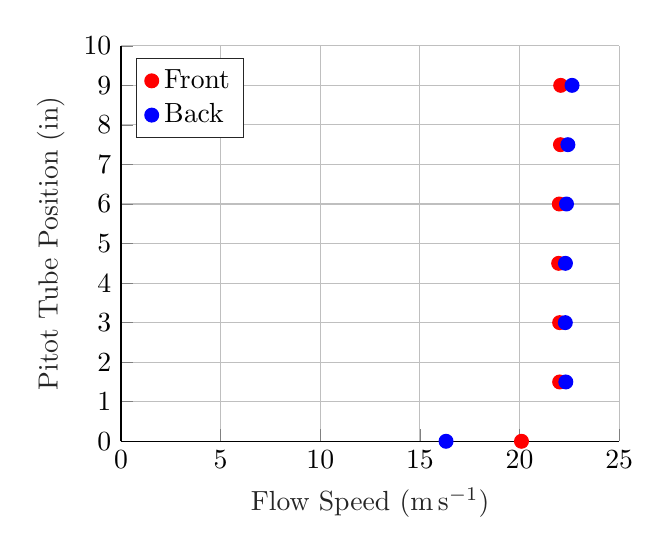
\begin{tikzpicture}

\begin{axis}[%
width=0.958\fwidth,
height=\fheight,
at={(0\fwidth,0\fheight)},
xmin=0,
xmax=25,
xlabel style={font=\color{white!15!black}},
xlabel={Flow Speed (\unit{\m\per\s})},
ymin=0,
ymax=10,
ylabel style={font=\color{white!15!black}},
ylabel={Pitot Tube Position (\unit{in})},
ytick={0,1,...,10},
axis background/.style={fill=white},
axis x line*=bottom,
axis y line*=left,
xmajorgrids,
ymajorgrids,
legend style={at={(0.03,0.97)}, anchor=north west, legend cell align=left, align=left, draw=white!15!black}
]
\addplot [color=red, only marks, mark size=2.5pt, mark=*, mark options={solid, red}]
  table[row sep=crcr]{%
20.09649115	0\\
22.01206383	1.5\\
22.01197829	3\\
21.96238566	4.5\\
21.99520315	6\\
22.053229	7.5\\
22.06480624	9\\
};
\addlegendentry{Front}

\addplot [color=blue, only marks, mark size=2.5pt, mark=*, mark options={solid, blue}]
  table[row sep=crcr]{%
16.310813	0\\
22.32169196	1.5\\
22.29623036	3\\
22.30278936	4.5\\
22.35630252	6\\
22.42566381	7.5\\
22.63432919	9\\
};
\addlegendentry{Back}

\end{axis}
\end{tikzpicture}%
    \caption{Velocity Profile at the front and back of the test section}
    \label{fig:vProfile}
\end{figure}

Fig.~\ref{fig:vProfile} shows that the air exhibited approximately uniform flow as expected.
The air appeared to be moving slower at the walls which indicates the presence of viscous forces~\cite{lecture}.
Classic aerodynamic theory indicates that the velocity at the wall should be zero.
The deviation between the experimental results and theory likely stems from the diameter of the Pitot tube creating an offset and preventing a true reading at the bottom wall of the test section.
This indicates that for future experiments, objects should be placed near the middle of the test section and away from the walls to have accurate readings of the flow speed.
It should be noted that due to the geometry of the Pitot-Static probe and the test section, a reading at the top wall of the test section could not be obtained.
One observation that can be made from Fig.~\ref{fig:vProfile} is that the velocities at the back of the test section were generally higher than those at the front.
This difference could have been due to heat addition from the ambient environment to the air inside the wind tunnel causing the flow to accelerate.
It was observed that the temperature of the ambient environment had gradually increased over the duration of the experiment.
This heat addition could have been due to the presence of people in the wind tunnel laboratory and the operation of the wind tunnels themselves adding heat to the flow in the test section.

\subsection{Flow Speed as a Function of Fan Setting}

As an additional point of investigation, the flow speeds that were derived from the recorded dynamic pressure were plotted against the various fan speed settings in \unit{\hertz}.
It was found that the relationship was approximately linear.
The data from Fig.~\ref{fig:Hz} indicates that the flow speed has a correlation to the fan setting, but only for a certain range of fan settings.
This presents a contrast to the tunnel calibration method which expressed a linear relationship for all fan settings that were measured.
Furthermore, this relationship may not be replicable for future experiments where models would be placed in the test section as the presence of models may disrupt the flow.
These observations point to the tunnel calibration method as a more appealing method of determing the flow speed.

\begin{figure}[H]
    \centering
    % This file was created by matlab2tikz.
%
%The latest updates can be retrieved from
%  http://www.mathworks.com/matlabcentral/fileexchange/22022-matlab2tikz-matlab2tikz
%where you can also make suggestions and rate matlab2tikz.
%
\definecolor{mycolor1}{rgb}{0.65098,0.65098,0.65098}%
%
\begin{tikzpicture}

\begin{axis}[%
width=0.958\fwidth,
height=\fheight,
at={(0\fwidth,0\fheight)},
xmin=0,
xmax=50,
xlabel style={font=\color{white!15!black}},
xlabel={Fan Setting (\unit{\hertz})},
ymin=0,
ymax=45,
ylabel style={font=\color{white!15!black}},
ylabel={Flow Speed (\unit{\m\per\s})},
ytick={0,5,...,45},
axis background/.style={fill=white},
axis x line*=bottom,
axis y line*=left,
xmajorgrids,
ymajorgrids
]
\addplot [color=black, only marks, mark size=2.5pt, mark=*, mark options={solid, black}, forget plot]
  table[row sep=crcr]{%
10	6.86\\
12.5	8.67\\
15	10.56\\
17.5	12.54\\
20	14.54\\
22.5	16.6\\
25	18.68\\
27.5	20.77\\
30	22.94\\
32.5	25.08\\
35	27.27\\
37.5	29.44\\
40	31.62\\
42.5	33.79\\
45	35.98\\
47.5	38.14\\
50	40.28\\
};
\addplot [color=mycolor1, line width=2.5pt, forget plot]
  table[row sep=crcr]{%
10	6.28490196078432\\
12.5	8.39458333333334\\
15	10.5042647058824\\
17.5	12.6139460784314\\
20	14.7236274509804\\
22.5	16.8333088235294\\
25	18.9429901960784\\
27.5	21.0526715686275\\
30	23.1623529411765\\
32.5	25.2720343137255\\
35	27.3817156862745\\
37.5	29.4913970588235\\
40	31.6010784313725\\
42.5	33.7107598039216\\
45	35.8204411764706\\
47.5	37.9301225490196\\
50	40.0398039215686\\
};
\end{axis}
\end{tikzpicture}%
    \caption{Relation between flow speed and fan setting after discarding the low-speed outlier data points.}
    \label{fig:Hz}
\end{figure}

\subsection{Reynolds Number in the Test Section}

To investigate whether the velocity profile measured in the test section aligns with theory, the Reynolds number was calculated using~\eqref{eq:Re}~\cite{HeatTransfer}, where $u$ is the fluid velocity, $d_h$ is the hydraulic diameter of the pipe, $\nu$ is the kinematic viscosity, and $Re$ is the Reynolds number.
\begin{equation} \label{eq:Re}
    Re = \frac{ud_h}{\nu}
\end{equation}
The fluid velocity was taken from the approximate center of the test section.
At the front of the test section at \qty{6}{in} position, the Reynolds number was calculated to be $438000 \pm 1547$. At the back of the test section, it was $444000 \pm 1571$. Both numbers are greater than the critical Reynolds number of about 2800, indicating that the flow is turbulent~\cite{HeatTransfer}. The velocity profile in Fig.~\ref{fig:vProfile} aligns with aerodynamic theory for turbulent pipe flow.


\section{Conclusion}


For the first part of the experiment, the value of the tunnel calibration coefficient was found to be $-0.600 \pm 0.002$.
The determination of the tunnel calibration coefficient will allow future experiments to determine the velocity of the flow without the use of a Pitot-static probe in the test section.
A measurement of the change in static pressure between the ambient environment and the test section can be interpolated with the tunnel calibration coefficient.
This interpolation provides a corresponding dynamic pressure, from which the flow velocity can be calculated.
For the second part of the experiment, the velocity profiles at the entrance and exit of the test section exhibited signs of uniform flow as predicted in the lecture~\cite{lecture}.
The observation that the flow velocities at the exit were slightly greater than those at the entrance indicated the presence of an external factor that was adding kinetic energy to the flow.
Another observation was that there was a measured non-zero velocity at the wall of the test section when theory of the no-slip condition indicates it should have been zero~\cite{Aero}.
This discrepancy was likely due to the diameter of the Pitot tube not allowing exact dynamic pressure measurements at the wall~\cite{Aero}.
For further experiments, additional mitigations like thermal insulation could be put into place to ensure steady adiabatic conditions that would help to reduce any systematic biases in the results.
Additionally, smaller increments for the velocity profile could serve to increase the accuracy of the velocity profile curve that is formed.
The velocity profile near the wall could be further improved through the utilization of laser Doppler anemometry, which would assist in obtaining accurate readings for velocities near the wall of the test section~\cite{PitotLecture}.  


\section*{Appendix A: Uncertainty Calculation}


\begin{table}[H]
    \centering
    \caption{Summary of Measurement Uncertainties}
    \begin{tabular}{cccc}
    \toprule
    Parameter & Symbol & Justification & Uncertainty \\ \midrule \midrule
    \makecell{Transducer \\ Calibration} & $\mu P_\text{ind}$ & \cite{transducer} & 0.5\% $P_\text{ind}$ \\
    \makecell{Manometer \\ Reading} & $\mu P_\text{man}$ & \makecell{Half of \\ interval} & \qty{0.05}{in\ce{H_2O}} \\
    Temperature & $\mu T$ & Digital & \qty{0.1}{\celsius} \\
    Humidity & $\mu \varphi$ & Digital & 1\% \\
    Ambient Pressure & $\mu P_\text{amb}$ & Barometer & \qty{0.02}{\mm} \\
    Dynamic Pressure & $\mu q$ & \makecell{95\% Conf. \\ Int.} & \makecell{Variable, \\ $\sim \qty{0.002}{in\ce{H_2O}}$} \\
    \makecell{Static Pressure \\ Difference} & $\mu \Delta P$ & \makecell{95\% Conf. \\ Int.} & \makecell{Variable, \\ $\sim \qty{0.002}{in\ce{H_2O}}$} \\
    \makecell{Tunnel Calibration \\ Slope} & $\mu m$ & Monte Carlo & 0.0006 \\
    \makecell{Tunnel Calibration \\ Coefficient} & $\mu K$ & RSS & 0.002 \\
    \makecell{Saturation \\ Pressure} & $\mu P_g$ & RSS & \qty{16}{\pascal} \\
    Density & $\mu \rho$ & RSS & \qty{0.004}{\kg\per\m\cubed} \\
    Fluid Velocity & $\mu V_\text{flow}$ & RSS & Variable, $\sim \qty{0.04}{\m\per\s}$ \\
    \makecell{Kinematic \\ Viscosity} & $\mu \nu$ & \cite{KViscosity} & \qty{0.00000002}{\m\squared\per\s} \\ \bottomrule
    \end{tabular}
    \label{tab:uncertainty}
\end{table}

The uncertainty for the Dynamic Pressure ($q$) and the Static Pressure Difference ($\Delta P$) was obtained using a 95\% confidence interval with a normal distribution.
A normal distribution was used instead of a student's $t$-distribution as the sample size of 5000 was deemed sufficiently large that the sample distribution approach the normal distribution due to the central limit theorem~\cite{MoMLecture}.
A $z^*$ value of 1.96 was used for the calculation of the 95\% confidence interval~\cite{MoMLecture}.
The margin of error then served as the uncertainty, where $\mu X$ is the margin of error for an arbitrary measurement, $S_x$ is the sample standard deviation, and $n$ is the number of samples~\eqref{eq:conf}.

\begin{equation} \label{eq:conf}
    \mu X = z^* \frac{S_x}{\sqrt{n}}
\end{equation}

The uncertainty for the tunnel calibration coefficient ($K$) can be calculated using error propagation theory~\cite{errorprop}, where $m$ is the tunnel calibration slope obtained from the line of best fit of the dynamic pressure vs. static pressure difference plot (Fig.~\ref{fig:data})~\eqref{eq:uK}.

\begin{equation} \label{eq:uK}
    \mu K = \mu m \frac{\partial K}{\partial m} = -\frac{\mu m}{m^2}
\end{equation}

The uncertainty for the saturation pressure ($P_g$) can be calculated using error propagation theory~\cite{errorprop}, where $T$ is the ambient temperature~\eqref{eq:uPsat}.

\begin{equation} \label{eq:uPsat}
    \mu P_g = \mu T \frac{\partial P_g}{\partial T}
\end{equation}

The uncertainty for the fluid density ($\rho$) can be calculated using the RSS method~\cite{MoMLecture}, where $P$ is the ambient pressure, $T$ is the ambient temperature, $\varphi$ is the relative humidity, and $P_g$ is the saturation pressure~\eqref{eq:uRho}.

\begin{equation} \label{eq:uRho}
    \resizebox{227pt}{!}{$\displaystyle{\mu \rho = \left[\left(\mu P \frac{\partial \rho}{\partial P}\right)^2 + \left(\mu T \frac{\partial \rho}{\partial T}\right)^2 + \left(\mu \varphi \frac{\partial \rho}{\partial \varphi}\right)^2 + \left(\mu P_g \frac{\partial \rho}{\partial P_g}\right)^2\right]^{1/2}}$}
\end{equation}

The uncertainty for the velocity of the fluid ($V_\text{flow}$) can be calculated using the RSS method~\cite{MoMLecture}, where $q$ is the dynamic pressure and $\rho$ is the fluid density~\eqref{eq:uV}.
The uncertainty, while technically a distinct value for each value of the fluid velocity, was consistently $\pm \qty{0.04}{\m\per\s}$ when rounded to the nearest hundredth.

\begin{equation} \label{eq:uV}
    \mu V_\text{flow} = \left[\left(\mu q \frac{\partial V_\text{flow}}{\partial q}\right)^2 + \left(\mu \rho \frac{\partial V_\text{flow}}{\partial \rho}\right)^2\right]^{1/2}
\end{equation}

The uncertainty for the Reynolds number of the fluid ($Re$) was calculated using the RSS method~\cite{MoMLecture}, where $u$ is the fluid velocity, $d_h$ is the hydraulic diameter of the pipe, $\nu$ is the kinematic viscosity, and $Re$ is the Reynolds number~\eqref{eq:uRe}.

\begin{equation} \label{eq:uRe}
    \resizebox{227pt}{!}{$\displaystyle{\mu Re = \left[\left(\mu \nu \frac{\partial Re}{\partial \nu}\right)^2 + \left(\mu u \frac{\partial Re}{\partial u}\right)^2 + \left(\mu d_h \frac{\partial Re}{\partial d_h}\right)^2\right]^{1/2}}$}
\end{equation}

\begin{thebibliography}{99}
    \bibitem{lecture} Abbitt, J. D., ``Wind Tunnel Operating Characteristics
    Wind tunnel Calibration,'' \textit{University of Florida E-Learning} [PowerPoint slides], URL: \url{https://ufl.instructure.com/courses/480244/files/80557995}, 2023.
    \bibitem{MoMLecture} Ridgeway, S., ``MOM\_lab Uncertainty basics w tension,'' \textit{University of Florida E-Learning} [PowerPoint slides], URL: \url{https://ufl.instructure.com/courses/447927/files/65674680}, 2022.
    \bibitem{calculator} Abbitt, J. D., and Ukeiley, L. S., ``Air density calculator.xlsx,'' \textit{University of Florida E-Learning} [Excel spreadsheet], URL: \url{https://ufl.instructure.com/courses/480244/files/77543966}, 2023.
    \bibitem{gravity} Thompson, A., and Taylor, B. N, ``Appendix B. Conversion Factors,'' \textit{Guide for the Use of the International System of Units (SI)}, National Institute of Standards and Technology, Maryland, 2008, p. 50.
    \bibitem{Aero} J. J. Bertin and R. M. Cummings, Aerodynamics for Engineers. Cambridge University Press, 2022.
    \bibitem{PitotLecture} Abbitt, J. D., ``HotWire-measurements,'' \textit{University of Florida E-Learning} [PowerPoint slides], URL: \url{https://ufl.instructure.com/courses/480244/files/77543976}, 2023.
    \bibitem{errorprop} Harry Ku (1966). Notes on the Use of Propagation of Error Formulas, J Research of National Bureau of Standards-C. Engineering and Instrumentation, Vol. 70C, No.4, pp. 263--273.
    \bibitem{transducer} MKS Baratron Type 223B Pressure Transducer User Manual, MKS Instruments, Inc., Anodver, MA, 1996.
    \bibitem{HeatTransfer} Bergman, T. L., and Lavine, A. S., ``Internal Flow,'' \textit{Fundamentals of Heat and Mass Transfer}, Wiley, New Jersey, 2017, p. 471.
    \bibitem{KViscosity} Bergman, T. L., and Lavine, A. S., ``Appendix A: Thermophysical Properties of Matter,'' \textit{Fundamentals of Heat and Mass Transfer}, Wiley, New Jersey, 2017, p. 911.
\end{thebibliography}

\end{document}